\chapter{Implementation \& Evaluation}
\label{ch:impl_eval}

\begin{comment}
\section{Baseline with MCTS}
In order to develop a non-trivial strategy for an enemy playing the game(s) developed in chapter \ref{ch:modelling}, we'll use  the MCTS algorithm described in section \ref{sec:intro_mcts}.
While we could use MCTS in stead of MARL algorithms, MCTS does have some properties that make it unsuitable for our purposes. Firstly, it uses the complete state information of the game. Secondly, while it generally outperforms simpler algorithms like minimax, it still doesn't scale to more realistic situations. Furthermore, since MCTS works on turn-based games, the game from chapter \ref{ch:modelling} is adapted to accommodate executing actions in sequence for the two players.\\

However, it does allow us to develop strategies for two opposing players form the ground up. Thus using MCTS at this phase has two purposes:
\begin{enumerate}
    \item Analyzing the performance of the algorithm
    \item Obtaining a baseline opponent policy against which the MARL algorithms can be evaluated.
\end{enumerate}

\end{comment}
% ----------------------------------------------------------------------------------------

%\section{Innateness vs. Learned}
%\textbf{Discuss advantages / disadvantages of innate knowledge (e.g. no aim/fire when not in range $\rightarrow$ might be valid initial knowledge, while simple strategies might not)} 

\section{Notes on implementation}
This section describes a couple of technical points about the implementation of the algorithms.
\begin{itemize}
    \item Because of the structure of the observation that the environment provides to an agent (see \ref{sec:first_model}), all (learning) agents can use the same network. This is known as \emph{weight sharing} and improves the sample efficiency since only one common network must be trained instead of a network per agent.
    \item This network takes as input a tensor constructed from the observation and puts it through a fully-connected layer. The output for this layer is than fed to a GRU. At every time step, the hidden state of the GRU is transformed via another fully-connected layer in to the policy and/or the estimated $V$ or $Q$-values, depending on the type of algorithm. The entire network for an actor-critic agent, which does both value estimation as policy prediction, is schematically represented in figure \ref{fig:agent_net}. 
    \begin{figure}[htp]
        \centering
        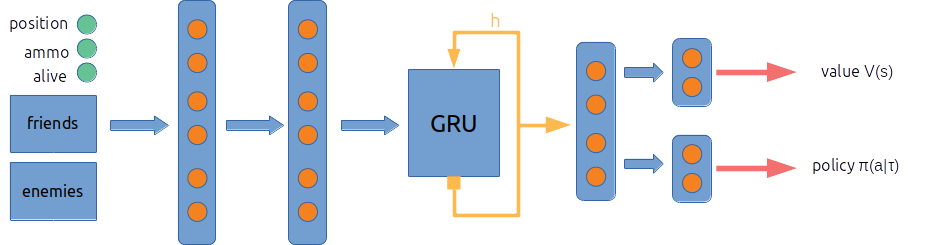
\includegraphics[width=14cm]{images/agent_net2.png}
        \caption{Actor-critic agent with a recurrent net}
        \label{fig:agent_net}
    \end{figure}
    \item \textbf{TODO}: how is this observation tensor constructed?
    \item
        The output of a policy network is an array of numbers, one per possible action, computed by the final linear policy layer. These so-called \emph{logits} $l_i$ are transformed into probabilities $p(a_i | s)$ via a softmax function:
        \begin{equation}
            p(a_i | s) = \frac{e^{l_i}}{\sum_j e^{l_j}}
        \end{equation}
    \item In multi-agent settings, agents that have died no longer contribute to the game and the only action at their disposal is the {\tt do\_nothing} action. Care has been taken that for observations and actions that correspond to situations where the agents are dead are not used for the update process.
    \item In Q-learning based algorithms like IQL and QMIX, the policy is created with an $\epsilon$-greedy action selection mechanism as described in section \ref{sec:deep_qn}. The $\epsilon$-term is responsible for the trade-off between exploration and exploitation. To assure enough exploration in the beginning, $\epsilon$ is typically reduced during training from its initial value of $1$ to a low final value like $0.05$. How this decrease of $\epsilon$ is done is determined by a scheduler which computes for each step in the learning process the correpsonding value of $\epsilon$. In this project, an linear scheduler has been used.
    \item Algorithms of the Q-learning family, like IQL and QMIX, have more hyperparameters than algorithms from the policy gradient family due to the presence of a replay buffer and a target network. These hyperparameters includes the buffer and batch size, as well as the target synchronisation rate and the $\epsilon$ decay rate. This implies that searching an optimal combination of parameters becomes exponentially more difficult.
    \item In order to account for random effects, the average of the different measurements should be computed over multiple runs. However, this would mean that runs have to be repeated several times and development would slow down significantly. For this reason, averages were computed by letting a window slide over a single run and averaging the measurements in this window. This can be justified by the fact that the learning rate is chosen small enough so that the weights of the network don't change significantly in this window. Technically, we assume that the signal is weakly stationary and the ergodic hypothesis thus holds.
    \item \ldots
\end{itemize}

\section{First Model}
\subsection{Independent RL}
\label{sec:iql_applied}
This section discusses the application of IQL and IAC (section \ref{sec:intro_deep_indep_rl}) to the simple battlefield model described in section \ref{sec:first_model}. Two agents were trained with IQL and IAC (in casu the simple REINFORCE algorithm) on a 7-by-7 board against two opposing players who made random moves. The maximum range for all players was $5$ steps, so agents have to learn to approach other agents before firing. All training episodes were limited to maximum 100 steps.\\

A comment on random opponents: agents that make random moves are indeed simple to beat; the final goal however is to work in an iterative fashion: 
\begin{enumerate}
    \item Train two agents against two random agents.
    \item Train two new agents against these two already trained agents until they can consistently beat them.
    \item Continue in this way until no more progress is made.
\end{enumerate}
The figures below summarize the results of the first point.\\
% Nov13_10-05-55_ideapad-pg smoothing 0.95
% Add (insert): run 171
% [21Jan20] -> experiment 3 - run 187

This paragraph describes the results for independent REINFORCE. The training of both agents was run for 50000 episodes, generated by sampling actions from the policy $\pi_i(a_t|s_t)$ and interacting with the environment. Figures \ref{fig:exp1_grad0} and \ref{fig:exp1_grad1} show how the $L2$-norm of each policy gradient $G_t \, \nabla_{\bm{\theta}} \ln \pi(A_t|S_t,\bm{\theta})$ evolves during training (see the REINFORCE algorithm \ref{algo:reinforce}) for both agents. This norm gives an indication how the gradient ascent algorithm changes the network parameters. Notice that while initially the gradient increases, it finally tops off and starts to decrease. Running the experiment longer will show both graphs converging to zero, meaning that the agents have reached their goal and are no longer learning.\\
\begin{figure}
\centering
\begin{minipage}{.5\textwidth}
  \centering
  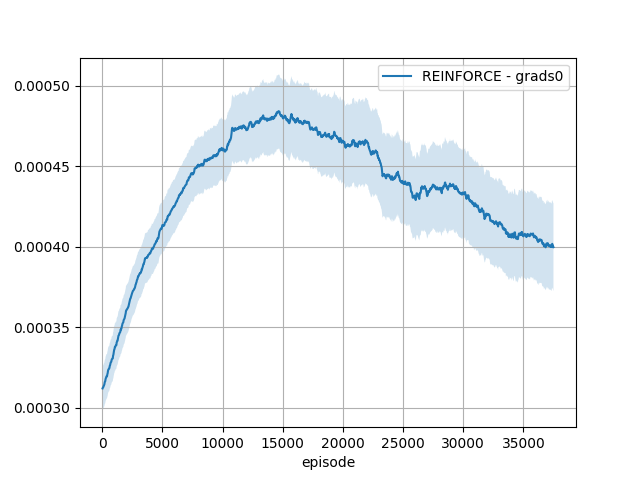
\includegraphics[width=8cm]{images/experiment4/grad0.png}
  \captionof{figure}{Gradient estimate for agent $0$}
  \label{fig:exp1_grad0}
\end{minipage}%
\begin{minipage}{.5\textwidth}
  \centering
  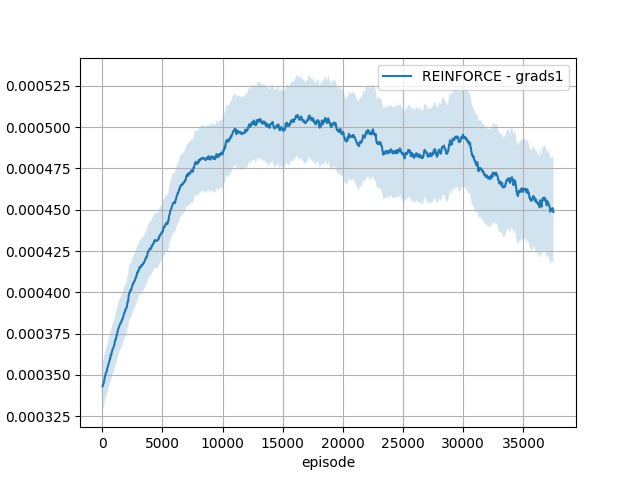
\includegraphics[width=8cm]{images/experiment4/grad1.png}
  \captionof{figure}{Gradient estimate for agent $1$}
  \label{fig:exp1_grad1}
\end{minipage}
\end{figure}

Figure \ref{fig:exp1_length} shows the average duration of an episode. Notice that initially, when the agent's policy network has random weights and he effectively functions as a random agent, the episodes take a long time because nobody is taking any directed actions. Once the agent's learns from experience, his behavior becomes more directive and the episode duration decreases rapidly. This behavior is stimualted by the fact that the agent receives a small negative reward for every step, incentivizing the agents to reduce the episode length. Figure \ref{fig:exp1_reward} shows the average final reward per episode for the agents. Initially, the agents lose as often as they win; the reward is negative, partially because agents are penalized for draws (e.g. because they run out of ammo). However, the win rate increases rapidly and finally the agents will win always all the time. This curve is called the \emph{learning curve} and will be the standard way to evaluate the performance of a MARL algorithm.\\

\begin{figure}
\centering
\begin{minipage}{.5\textwidth}
  \centering
  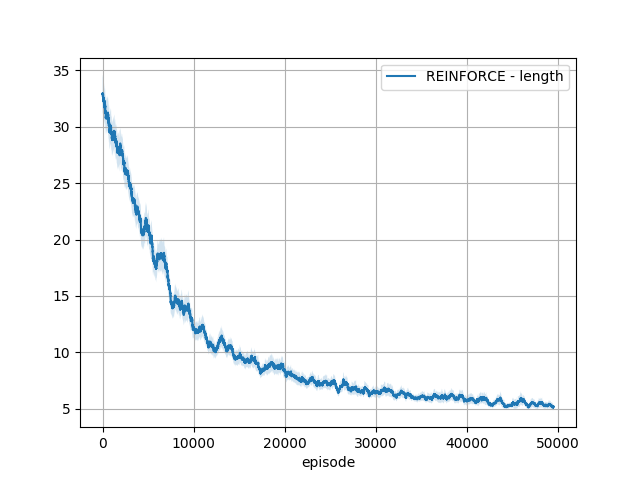
\includegraphics[width=8cm]{images/experiment4/mean_length.png}
  \captionof{figure}{Mean episode length}
  \label{fig:exp1_length}
\end{minipage}%
\begin{minipage}{.5\textwidth}
  \centering
  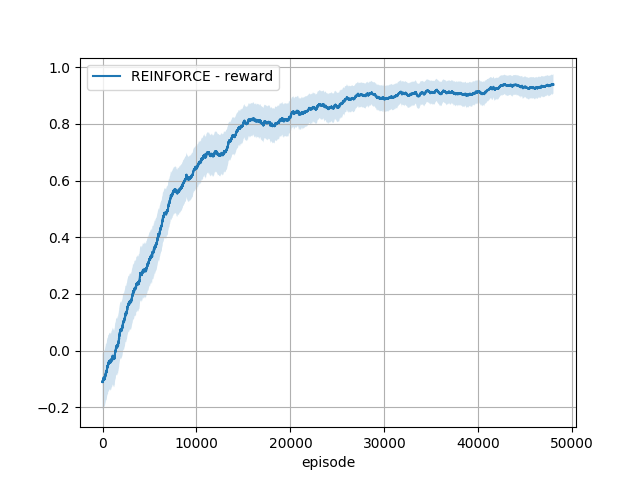
\includegraphics[width=8cm]{images/experiment4/mean_reward.png}
  \captionof{figure}{Mean reward for agents of team 1}
  \label{fig:exp1_reward}
\end{minipage}
\end{figure}

In this simple scenario, the agents have learned to (in this order):
\begin{enumerate}
    \item Aim at the opposing agents (resp. $0 \rightarrow 2$ and $1 \rightarrow 3$).
    \item Come closer until the opposing agent is in range.
    \item Fire once the opposing agent is in range.
\end{enumerate}
Figure \ref{fig:simple_tactic01} shows how this is done. A white line between agents means one agent is aiming at the other. The actions undertaken by the four agents is shown in the top left corners.

%\includemovie{8cm}{8cm}{images/tactic01.gif}
% \begin{frame}{}
%   \animategraphics[loop,controls,width=10cm]{10}{images/animation01/screenshot0-}{0}{4}
% \end{frame}

% \begin{frame}
%     \transduration<0-4>{0}
%     \multiinclude[<+->][format=png, graphics={width=10cm}]{images/animation01/screenshot0}
% \end{frame}

\begin{figure}
\centering
\begin{minipage}{.5\textwidth}
  \centering
  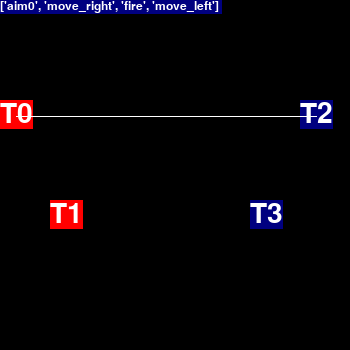
\includegraphics[width=7cm]{images/animation01/screenshot0-1.png}
\end{minipage}%
\begin{minipage}{.5\textwidth}
  \centering
  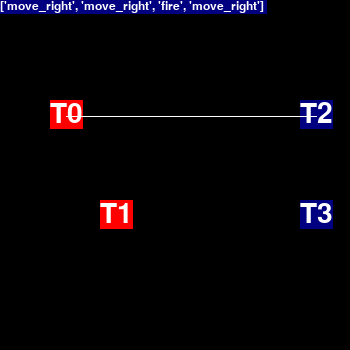
\includegraphics[width=7cm]{images/animation01/screenshot0-2.png}
\end{minipage}
%\end{figure}
%\begin{figure}
\centering
\begin{minipage}{.5\textwidth}
  \centering
  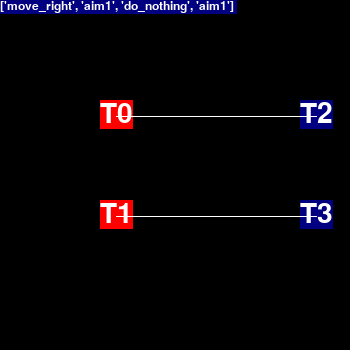
\includegraphics[width=7cm]{images/animation01/screenshot0-3.png}
\end{minipage}%
\begin{minipage}{.5\textwidth}
  \centering
  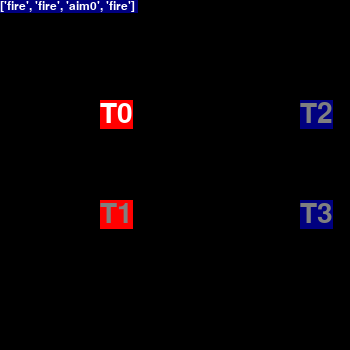
\includegraphics[width=7cm]{images/animation01/screenshot0-4.png}
\end{minipage}
\caption{A simple learned tactic}
\label{fig:simple_tactic01}
\end{figure}

\textbf{To mention}: use of optimizer (\emph{ADAM}) and learning rate.\\

Next, we compare the learning curves of the three types of independent learning algorithms: (i) REINFORCE, (ii) Independent Actor-Critic (IAC) and (3) Independent Q-Learning (IQL). The resulting learning curves are represented in figure \ref{fig:compare_reward} for games where 2 learning agents play against 2 random agents.

\begin{figure}[htp]
    \centering
    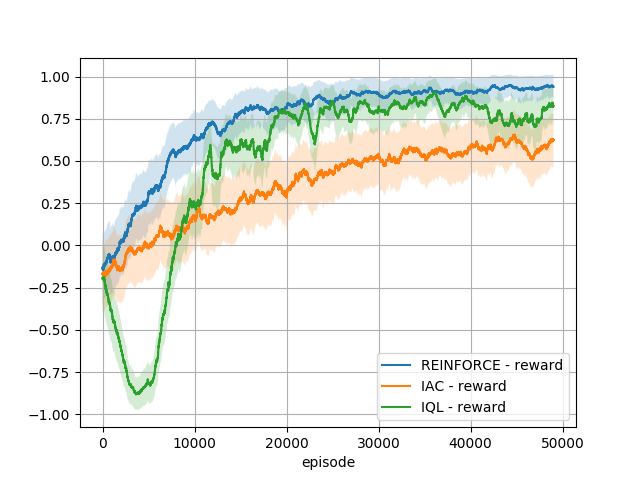
\includegraphics[width=14cm]{images/experiment4/compare_reward.png}
    \caption{Learning rate for REINFORCE, IAC and IQL for 2v2 games}
    \label{fig:compare_reward}
\end{figure}

The following points are significant:
\begin{itemize}
    \item Out of the 3 algorithms, REINFORCE works best.
    \item IQL initially goes in the wrong direction (i.e. makes wrong moves) before starting to improve the reward. This is caused by the high initial $\epsilon$ in the $\epsilon$-greedy action selection process which causes the behavior to be random instead of guided by the learned $Q$-values.
    \item Since IQL derives the policy from the learned $Q$-values, its behavior during learning undergoes significantly higher variation than REINFORCE.
    \item The learning curve of IAC is slower than those for REINFORCE and IQL. This is probably because IAC has to learn both a policy and value-estimation function at the same time.
    \item IAC is highly dependent on the inclusion of an entropy-term to avoid the policy distribution from collapsing to a distribution thet puts all probability mass on a single action.
\end{itemize}

Since REINFORCE works best, we'll use this algorithm to compare against QMIX, a true multi-agent algorithm.

\begin{comment}
\textbf{TODO:} Rephrase the paragraph below.\\
The next evolution is to represent the agent as a recurrent neural network as explained in section \ref{sec:deep_pg}. The input of the network are the two major components of the state vector $\bm{s_t}$:
\begin{enumerate}
    \item The game board, namely the actual position of the agent relative to the board and each other, and
    \item Additional information about the agents (are they alive? What is the ammo level?)
\end{enumerate}
The board information is well suited to serve as input of a convolutional layer, since it contains spatial information. The additional information on the other hand will be fed to a fully-connected neural network layer. The result of both these layers is then combined and serves as the input for the a fully-connected layer. The output of this layer is then fed to a GRU. The neural net will have two heads, as explained in section \ref{sec:deep_pg}, and can thus be used in an actor-critic algorithm. An overview of the agent's neural network is shown in figure \ref{fig:agent_net}.
\begin{figure}[htp]
    \centering
    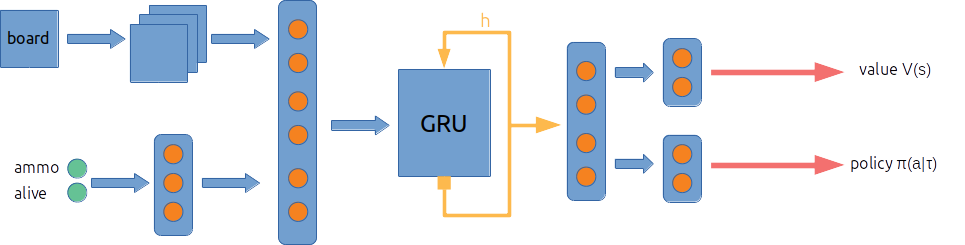
\includegraphics[width=16cm]{images/agent_net.png}
    \caption{Actor-critic agent with recurrent net}
    \label{fig:agent_net}
\end{figure}

While this modification might result in a theoretical improvement, this is not the case in practice. Figure \ref{fig:newplot194_195} shows the learning curve for agents with non-recurrent (blue) and recurrent neural nets (green). While both learn a winning strategy, it is not feasible to say one approach is better than the other. \textbf{TODO}: improve this (correct or explain).

% comparison 194-195
\begin{figure}[htp]
    \centering
    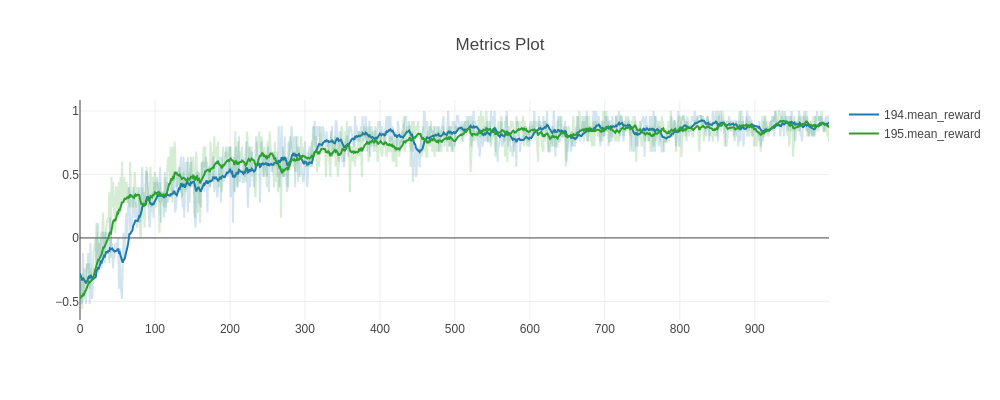
\includegraphics[width=14cm]{images/experiment2/newplot194_195.png}
    \caption{Forward vs. GRU Network}
    \label{fig:newplot194_195}
\end{figure}

%insert comparison PG (run ideapad 582) and IQL (run ideapad 590)
\end{comment}

\subsection{QMIX}
As explained in section \ref{sec:intro_qmix}, QMIX is an algorithm of the Q-learning family that combines the Q-value estimate of the different agents into a $Q_{tot}$ such that $\frac{\partial Q_{tot}}{\partial Q_i} \geq 0$ for all agents $i$. This guarantees that when each agent chooses his best action $a_i$, the combined action set $[a_1 \ldot a_N]$ will also be the best possible joint action for the team.\\
QMIX uses during training the state information $s_t$ to set the weights of the mixing network in figure \ref{fig:qmix_structure}. To do this, the state information was transformed in a tensor of size {\tt n\_agents x 5}, where each agent is represented by 5 items: his position $(x, y)$, whether he is still alive, his ammo level and at whom he is aiming (if any).\\
Figure \ref{fig:comp_qmix_pg} compares the learning curve of REINFORCE with the one for QMIX.
% comparison 396-419
\begin{figure}[htp]
    \centering
    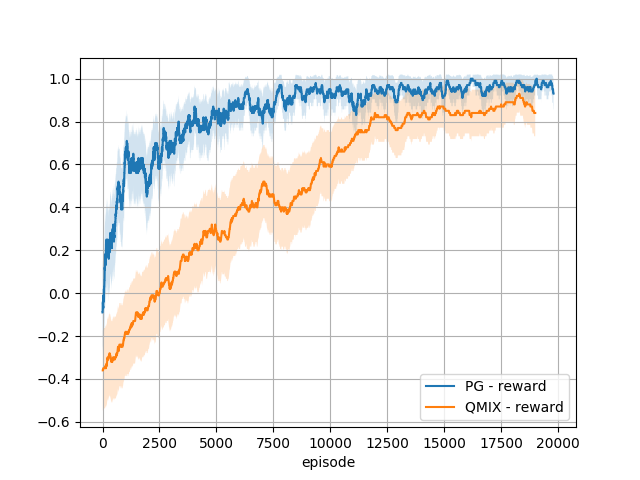
\includegraphics[width=16cm]{images/experiment5/pg_v_qmix_simple.png}
    \caption{QMIX vs independent REINFORCE in a simple environment}
    \label{fig:comp_qmix_pg}
\end{figure}
Clearly, independent REINFORCE works better, both in sample efficiency (since its curve is steeper) and in final result. However, QMIX is an algoritm better suited to complexer situations, thus its advantages should become more clear when we look at more complex environments.

\section{Second Model}
\subsection{Independent RL}
\subsection{QMIX}

\section{Model Transfer}
% TODO: explain model transfering from friend to foe
% TODO (maybe) discuss transferability over different terrains